\documentclass[10pt]{article}
\usepackage{icmlko}

\icmlmeta{IP 파운데이션 월드모델}{71}{판정하던 자와 파는 물건이 달랐다}{서른여덟 노트 동안 셀별 전이의 평균으로 판정했는데 제품이 쓰는 것은 출처를 합친 앙상블이다}

\begin{document}

\twocolumn[
\icmlheader

\begin{abstract}
노트 33부터 일흔까지 판정치는 줄곧 \textbf{셀별 전이의 평균}이었다 --- ``출처
하나로 대상 하나를 얼마나 맞히나.'' 제품이 쓰는 것은 그게 아니다 --- ``\textbf{가진
것 전부로} 대상 하나를 맞히면 얼마나 맞나.'' 둘을 나란히 쟀다. \textbf{앙상블이
일곱 대상 전부에서 이긴다.} 팝업이 $+$0.3263에서 \textbf{$+$0.4685}로($\Delta+$0.1340
{[}$+$0.072, $+$0.194{]}), 전체가 $+$0.1797에서 $+$0.2612로 오른다. 여섯 대상
모두 짝지은 구간이 0을 넘는다. 그리고 앙상블은 \textbf{최선 단일 출처($+$0.4762)에
거의 닿는다} --- 라벨 없이는 어느 출처가 최선인지 못 고르는데 합치면 공짜로
거기 간다. 팝업 출처 여섯 중 하나(애니)가 $-$0.3096으로 \emph{반대}를 가리키는데도
앙상블이 안 무너진다. \textbf{그래서 과거 판정을 다시 했다} --- 넷 중 하나가
뒤집힌다(노트 48 웹툰 굿즈 배선: 보류 $\to$ 되돌리기 채택). 예상이 하나 빗나갔다
--- 앙상블이 방향 결정을 \emph{싸게} 만들 줄 알았는데 \textbf{더 비싸게} 만든다.
결정이 여섯에서 하나로 줄어 헤지가 사라지기 때문이며, $k{=}32$에서도 구간이
0을 포함한다. 마지막으로 제품 수치의 구간을 처음 쟀다 --- \textbf{6.13배
{[}2.12, 10.98{]}}. 순위는 확실히 좋아졌고 \textbf{배수는 아직 말할 수 없다}.
\end{abstract}
]

\section{두 개의 자}

\begin{quote}\fontsize{9.5}{11.5}\selectfont
\textbf{연구 질문} 게임으로 팝업을 맞히면 얼마나 맞나 --- 42셀 평균.\\
\textbf{제품 질문} \textbf{가진 것 전부로} 팝업을 맞히면 얼마나 맞나 --- 앙상블.
\end{quote}

노트 58 · 59가 낸 제품 수치는 이미 다섯 출처를 합쳐 냈다. 그러니까 \emph{제품
수치는 틀리지 않았다}. 틀린 것은 \textbf{판정 척도}다 --- 배선 · $\lambda$ · 축
결정 서른 몇 개를 전부 셀 평균으로 재고 있었다.

\paragraph{순위로 합친다}
출처마다 예측의 눈금이 다르므로(노트 59가 눈금 보정을 따로 다룬 이유다) 값이
아니라 순위를 평균한다. 가중치는 안 준다 --- 출처의 자기 상관으로 가중하면
노트 38 · 40의 상충 법칙 때문에 오히려 나쁜 출처에 힘이 실린다. z 평균과
순위 평균은 사실상 같다(일곱 대상 최대 차 0.008). \textbf{어떻게 합치느냐가
아니라 합치느냐가 문제다.}

\section{일곱 대상 전부에서 이긴다}

\begin{figure*}[t]
\centering
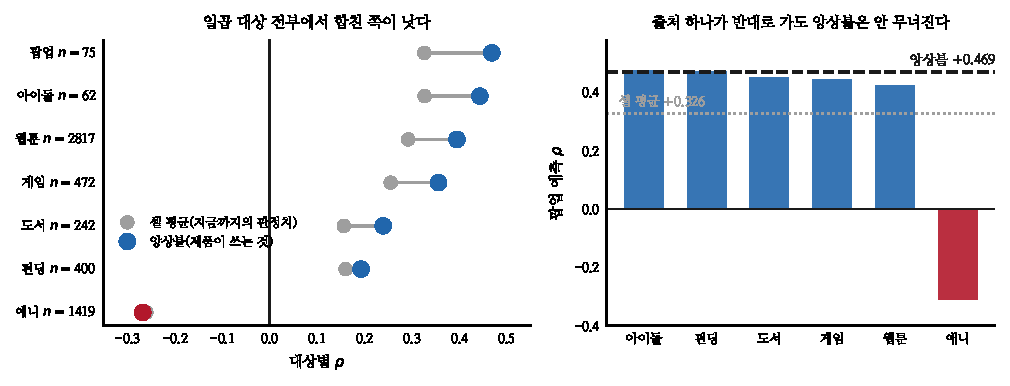
\includegraphics[width=\textwidth]{figs/together.pdf}
\caption{왼쪽 --- 대상별 셀 평균과 앙상블. 오른쪽 --- 팝업의 출처별 성적.}
\end{figure*}

\begin{table}[t]
\centering\tsize
\caption{대상별. 짝지은 붓스트랩 400회.}
\begin{tabular}{lrrrl}
\toprule
대상 & 셀 평균 & 앙상블 & $\Delta$ & 95\% 구간 \\
\midrule
팝업 & $+$0.3263 & \textbf{$+$0.4685} & $+$0.1340 & $[+0.072, +0.194]$ \\
아이돌 & $+$0.3269 & $+$0.4433 & $+$0.1159 & $[+0.048, +0.178]$ \\
웹툰 & $+$0.2923 & $+$0.3951 & $+$0.1027 & $[+0.094, +0.111]$ \\
게임 & $+$0.2555 & $+$0.3562 & $+$0.0996 & $[+0.074, +0.123]$ \\
도서 & $+$0.1567 & $+$0.2397 & $+$0.0816 & $[+0.038, +0.121]$ \\
펀딩 & $+$0.1604 & $+$0.1929 & $+$0.0325 & $[+0.013, +0.055]$ \\
애니 & $-$0.2599 & $-$0.2674 & $-$0.0076 & $[-0.010, -0.005]$ \\
\midrule
전체 & $+$0.1797 & $+$0.2612 & & \\
\bottomrule
\end{tabular}
\end{table}

여섯 대상 전부 구간이 0을 넘는다. 애니만 음수인데 그것은 방향이 뒤집힌 상태라
앙상블이 \emph{일관되게} 반대로 간다는 뜻이다 --- 합치기가 실패한 게 아니다.

\claimx{판정치를 셀 평균에서 앙상블로 바꾼다. 제품이 쓰는 것이 그것이고, 일곱
대상 전부에서 더 높으며, 여섯에서 짝지은 구간이 0을 넘는다.}{앙상블은 출처가
많을수록 유리하므로 도메인 수에 더 민감하다. 도메인이 적은 초기 노트와
비교할 때는 눈금이 다르다.}

\section{반대로 가는 출처가 있어도 안 무너진다}

\begin{table}[t]
\centering\tsize
\caption{팝업을 맞히는 출처 여섯.}
\begin{tabular}{lr}
\toprule
아이돌 & $+$0.4762 \\
펀딩 & $+$0.4729 \\
도서 & $+$0.4497 \\
게임 & $+$0.4451 \\
웹툰 & $+$0.4234 \\
\textbf{애니} & \textbf{$-$0.3096} \\
\midrule
셀 평균 & $+$0.3263 \\
\textbf{앙상블} & \textbf{$+$0.4685} \\
\bottomrule
\end{tabular}
\end{table}

여섯 중 하나가 반대를 가리키는데 앙상블이 $+$0.4685다. 최선 단일($+$0.4762)에
1.6\% 차이로 닿는다. \textbf{어느 출처가 최선인지는 대상 라벨 없이 못 고른다.
앙상블은 그 선택을 안 해도 되게 만든다.}

애니를 아예 빼면 $+$0.4703, 부호를 뒤집어 넣으면 $+$0.4528이다. 셋이 전부
$\pm$0.02 안에 있다 --- \textbf{나쁜 출처를 어떻게 처리하든 차이가 없다.}

\section{과거 판정을 다시 했다}

\begin{table}[t]
\centering\tsize
\caption{같은 결정, 두 자. 하나가 뒤집힌다.}
\begin{tabular}{lll}
\toprule
결정(되돌리는 방향) & 셀 평균 & 앙상블 \\
\midrule
도서 타깃 폭 끄기 & 악화 & 악화 \\
게임 고유 축 떼기(노트 54) & 악화 & 악화 \\
\textbf{웹툰 굿즈 되돌리기(노트 48)} & \textbf{보류} & \textbf{채택} \\
애니 방향 뒤집기(노트 69) & 채택 & 채택 \\
\bottomrule
\end{tabular}
\end{table}

넷 중 셋은 그대로다. 하나가 뒤집힌다 --- 노트 48이 웹툰 굿즈 규모를 연재 밀도에서
참여 작가 수로 바꾼 결정인데, 앙상블 자로 재면 \textbf{되돌리는 쪽이 채택}이다
($+$0.0132 {[}$+$0.0032, $+$0.0286{]}). 노트 67이 이미 ``표본이 세 배가 되자
사라졌다''고 적었던 그 결정이며, 이제 자를 바꾸니 \emph{반대로} 판정된다.

\claimx{판정 척도를 바꾸면 결정이 바뀐다 --- 넷 중 하나가. 셀 평균으로 내린
과거 판정 전부가 재검토 대상이다.}{넷만 다시 쟀다. 나머지를 다 재려면 계산이
크고, 대부분은 효과가 반폭 아래라 어차피 보류로 나올 것이다.}

\section{예상이 빗나갔다 --- 앙상블은 방향을 더 비싸게 만든다}

\begin{table}[t]
\centering\tsize
\caption{앙상블의 방향을 $k$건으로 정한다(노트 70과 같은 유보 규약).}
\begin{tabular}{lrl}
\toprule
$k$ & $\Delta$ & 95\% 구간 \\
\midrule
2 & $-$0.1906 & $[-0.411, +0.076]$ \\
8 & $-$0.0916 & $[-0.352, +0.077]$ \\
16 & $+$0.0001 & $[-0.147, +0.078]$ \\
32 & $+$0.0496 & $[-0.073, +0.078]$ \\
\bottomrule
\end{tabular}
\end{table}

노트 70에서 셀별 부호는 $k{=}32$에 채택됐다. 앙상블은 $k{=}32$에도 구간이 0을
포함한다. 이유가 분명하다 --- 셀별은 대상마다 여섯 번 결정하고 앙상블은 \textbf{한
번} 결정한다. 여섯 번 중 넷만 맞아도 평균이 살아남지만, 한 번 틀리면 대상 전체가
뒤집힌다.

\claimx{합치기는 \emph{예측}을 좋게 하고 \emph{방향 결정}을 나쁘게 한다. 평균이
잡음을 줄이는 것과 같은 이유로 방향 오판의 헤지도 함께 사라진다.}{앙상블 부호를
셀별 부호의 다수결로 정하면 둘 다 얻을지 모른다. 안 해 봤다.}

\section{제품 수치에 구간을 붙인다}

\begin{table}[t]
\centering\tsize
\caption{팝업 예측 상하위 20\% 일평균 방문자 배수. 붓스트랩 600회.}
\begin{tabular}{lrl}
\toprule
& 배수 & 95\% 구간 \\
\midrule
\textbf{앙상블 여섯} & \textbf{6.13} & $[2.12,\ 10.98]$ \\
최선 단일(아이돌) & 5.24 & $[2.41,\ 10.91]$ \\
\midrule
\multicolumn{2}{l}{앙상블 $-$ 개별 평균 ($\log_{10}$ 배수)} &
$+0.201\ [-0.051, +0.378]$ \\
\bottomrule
\end{tabular}
\end{table}

노트 58이 5.5배라고 적은 이래 이 수치에 구간을 붙인 적이 없다. 붙여 보니
\textbf{{[}2.12, 10.98{]}}이다. 팝업이 75건이고 각 구간이 15건이라 그렇다.
짝지은 차이도 0을 포함한다.

\begin{quote}\fontsize{9.5}{11.5}\selectfont
\textbf{순위는 확실히 좋아졌고 배수는 아직 말할 수 없다.} 순위 상관은 75건
전부를 쓰지만 배수는 양 끝 15건씩만 쓴다. ``6.13배''를 제품 문구로 쓰면 안 되고,
쓸 수 있는 것은 여전히 노트 59의 문장이다 --- \emph{어느 기획을 먼저 밀지 고르는
데는 쓸 수 있고, 몇 명 올지 약속하는 데는 아직 못 쓴다.}
\end{quote}

\section{한계}

\begin{itemize}[leftmargin=1.1em,itemsep=0.15em]
\item 앙상블을 정본 파이프라인의 기본 판정치로 바꾸지 않았다. \texttt{audit}에
      \texttt{rho\_ens}를 넣어 둘 다 잴 수 있게만 했다.
\item 과거 결정 넷만 다시 쟀다.
\item 배수의 구간이 너무 넓어 앙상블이 배수를 올렸는지 모른다. 팝업 표본이
      늘기 전에는 못 좁힌다.
\item 애니가 방향이 뒤집힌 채로 들어가 있다. 노트 70이 문턱 32건을 냈지만
      정본에 아직 안 넣었다.
\item 앙상블 가중치를 균등으로 고정했다. 라벨 몇 건으로 가중치를 정하는 것은
      안 해 봤다.
\end{itemize}

\section{다음}

\begin{enumerate}[leftmargin=1.3em,itemsep=0.15em]
\item 판정치를 앙상블로 바꾸고 파이프라인 출력을 다시 낸다.
\item 앙상블 부호를 셀별 다수결로 정해 본다 --- 예측 이득과 방향 헤지를 둘 다
      얻는지.
\item 노트 48 웹툰 굿즈 배선을 되돌린다(앙상블 자로 채택됐다).
\item 여덟째 도메인. 앙상블은 출처가 많을수록 유리하므로 도메인 추가의 값이
      셀 평균으로 볼 때보다 크다.
\end{enumerate}

\vspace{0.6em}
\hrule height 0.3pt
\vspace{0.5em}
{\footnotesize
\textbf{참고문헌}\\[0.3em]
Breiman, L. (1996). Bagging predictors. \emph{Machine Learning}, 24(2), 123--140.\\[0.15em]
Dietterich, T. G. (2000). Ensemble methods in machine learning.
\emph{MCS}, 1--15.\\[0.15em]
Caruana, R. et al. (2004). Ensemble selection from libraries of models.
\emph{ICML}, 18.\\[0.15em]
Kuncheva, L. I., Whitaker, C. J. (2003). Measures of diversity in classifier
ensembles. \emph{Machine Learning}, 51(2), 181--207.\\[0.15em]
Efron, B., Tibshirani, R. J. (1993). \emph{An Introduction to the Bootstrap}.
Chapman \& Hall.
}

\end{document}
